\chapter{Introduction}
\section{Background and research purpose}
In the foreseeable future, the electrification of ocean systems, renewable ocean power sources and ocean energy networks will be necessary, which will help accelerate the growth and deployment of ocean renewable energy and ways to explore and understand the ocean [1]. To achieve electrification in the ocean, it is necessary to deploy corresponding sensor networks underwater and process the data received by underwater sensors in a timely manner. At the same time, underwater sensors are also an important tool for studying the marine environment. They can easily and flexibly explore underwater terrain and ecological environment, which provides convenience for the deployment of underwater sensor networks. A good underwater AUV needs to have good equipment waterproofness, long-distance underwater controllability and durability. For the water resistance of the equipment, we can use high-performance waterproof and pressure-resistant materials. The remote controllability needs to solve the problems of long-distance underwater communication. The durability of electrical equipment requires low energy consumption AUV and high-energy batteries or continuous equipment. Energy supply. Sufficient energy supply can keep underwater sensors and AUV equipment in an efficient and stable working state for a long time. Reducing human interference when electrical equipment is working underwater can also improve work efficiency and reduce deployment costs. Therefore, the energy supply for underwater electrical equipment has become a novel research direction. Such methods can solve the energy supply problem of underwater equipment economically and ensure the system to perform long-term and stable work [3]. In traditional marine engineering, power is supplied to underwater equipment through wet plug-in interfaces [4]. For the traditional wet plug interface technology, its high cost, complex docking method, poor safety performance, and easy to be corroded by seawater, make its disadvantages in marine engineering increasingly obvious. Wireless Power Transfer (WPT) simplifies the connection between underwater equipment and power supply, reduces the continuous operating cost of underwater equipment, saves a lot of resources, and gradually gains the favor of scholars.

The ocean itself and its surroundings contain a lot of energy, such as tidal energy, wave energy, ocean current energy, sea temperature difference energy, and sea salt difference energy. Ocean energy is rich, widely distributed, clean and pollution-free, but low energy density and strong regionality. These advantages make it attractive as a grid-connected energy, and may also make it an isolated and remote ocean energy source, thereby providing a valuable source of ocean space. Continuous development provides power solutions that are attractive. The rapid development of distributed ocean energy applications (such as underwater sensor networks, ocean sensors and monitoring technologies, ocean automatic network buoys, and deep sea and tsunami buoys) is beneficial. In particular, it can power an autonomous underwater vehicle (AUV) whose service life is limited by its battery power.

\begin{figure}[htbp]
    \centering
    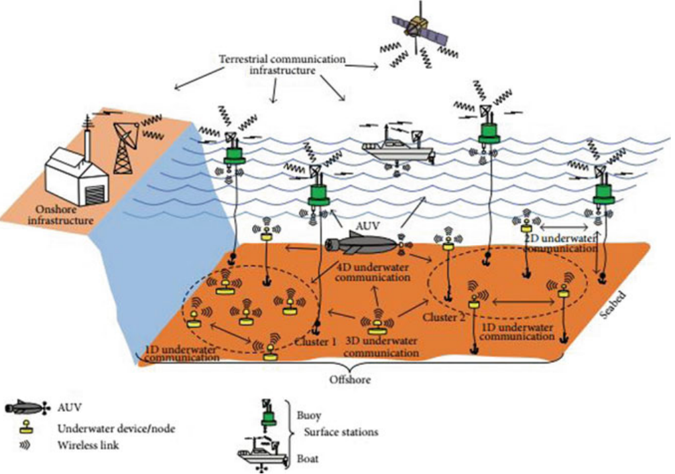
\includegraphics[width=0.9\linewidth]{images/1_underwater_sensor_networks.png}
    \caption{Underwater sensor networks architecture \cite{Nayyar}.}
\end{figure}

% \begin{figure}[htbp]
%     \centering
%     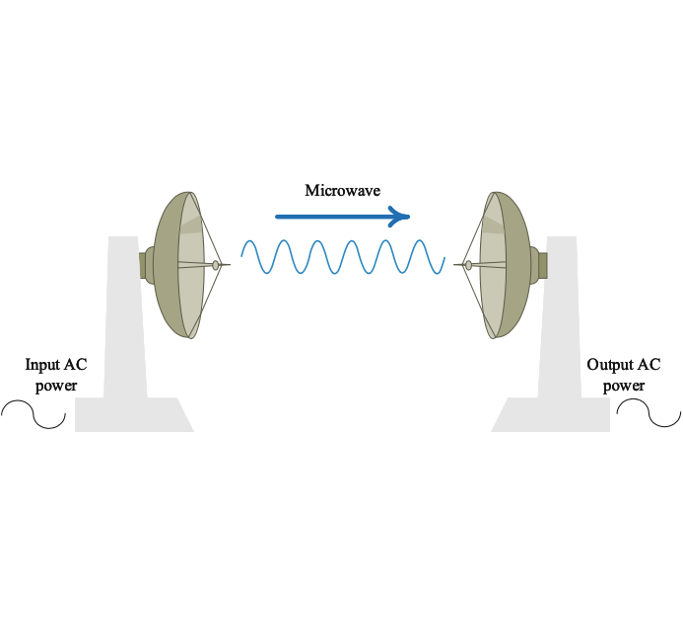
\includegraphics[width=150pt]{images/1_microwave_power_transfer.png}
%     \caption{Microwave power transfer.}
% \end{figure}
% \begin{figure}[htbp]
%     \centering
%     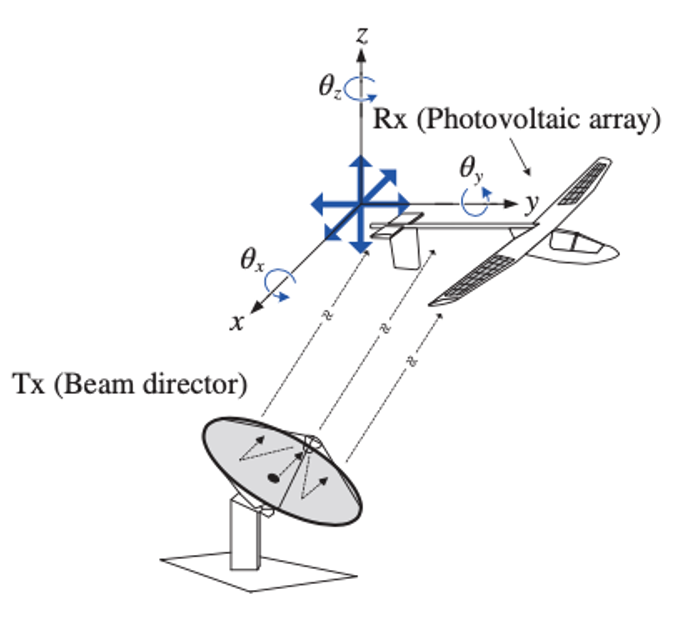
\includegraphics[width=150pt]{images/1_laser_power_transfer.png}
%     \caption{Laser power transfer.}
% \end{figure}


\section{Wireless power transfer technologies}

Broadly speaking, energy transmission without direct "electrical contact" between the primary and secondary is wireless energy transmission. Wireless energy technology can be divided into two main categories, Near-field (nonradiative region) power transfer and Far-field (radiative region) power transfer. 
Near-field means the area within about 1 wavelength ($\lambda$) of the antenna.  The range of near-field devices is conventionally divided into two categories:
\begin{itemize}
    \item  Short range – up to about one antenna diameter: $D_{range} \leq D_{ant}$.
    \item Mid-range – up to 10 times the antenna diameter: Drange $\leq$ 10 Dant.
  \end{itemize} 

Long-distance wireless energy transmission includes microwave, light, and sound wireless energy transmission. Short-distance wireless energy transmission includes short-distance magnetic field transmission using inductive coupling or electric field using capacitive coupling transmission. The respective characteristics are shown in the table ~\ref{table:differentWPT}.

\begin{table}[htbp]
    \centering
    \caption{The different wireless power technologies.}
    \begin{tabular}{ |c|c|c|m{3.5cm}<{\centering}|m{3.5cm}<{\centering}| }
        % \thickhline
        \hline
        \textbf{Technology} & \textbf{Range} & \textbf{Frequency}         & \textbf{Antenna devices}                    & \textbf{Applications}                             \\\hline
        % \thickhline
Microwaves          & hm - km        & GHz                        & Parabolic dishes, phased arrays, rectennas  & Satellite, drone aircraft                         \\ \hline
Optical             & dam - km
                    & $\geq$THz      & Lasers, photocells, lenses & Drone aircraft, space elevator                                                                  \\ \hline
Capacitive          & cm - m         & kHz – MHz                  & Metal plate electrodes                      & Smartcards, biomedical implant
\\ \hline
Inductive           & mm - m         & Hz – GHz                   & Tuned wire coils, lumped element resonators & Electric toothbrush, smartphone, electric vehicle
\\ \hline
    \end{tabular}
    \label{table:differentWPT}
\end{table}



\begin{figure}[htbp]
    \begin{subfigure}{0.5\textwidth}
        \centering
        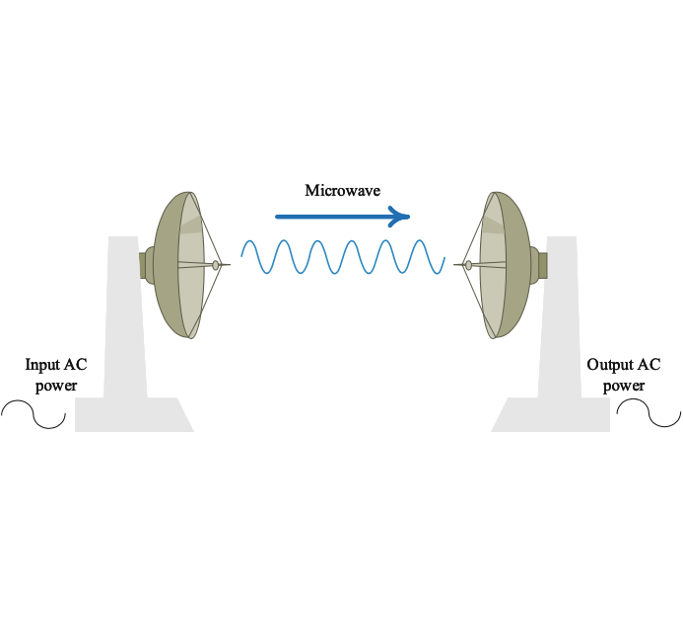
\includegraphics[width=0.9\linewidth]{images/1_microwave_power_transfer.png}
        \caption{Microwave power transfer \cite{Orekan}.}
        \label{fig:subim1}
    \end{subfigure}
    \begin{subfigure}{0.5\textwidth}
        \centering
        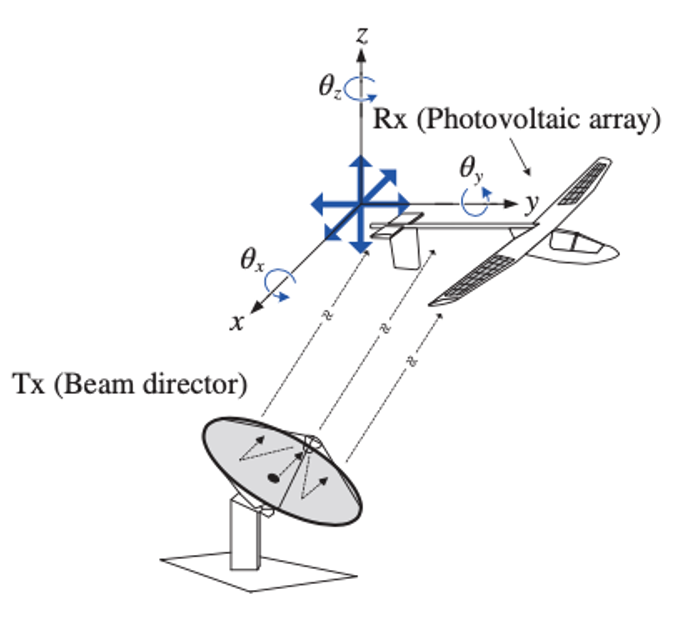
\includegraphics[width=0.9\linewidth]{images/1_laser_power_transfer.png}
        \caption{Laser power transfer \cite{Chun}.}
        \label{fig:subim2}
    \end{subfigure}

    \caption{Far-field wireless power transfer.}
    \label{fig:image2}
\end{figure}

\begin{figure}[htbp]
    \begin{subfigure}{0.5\textwidth}
        \centering
        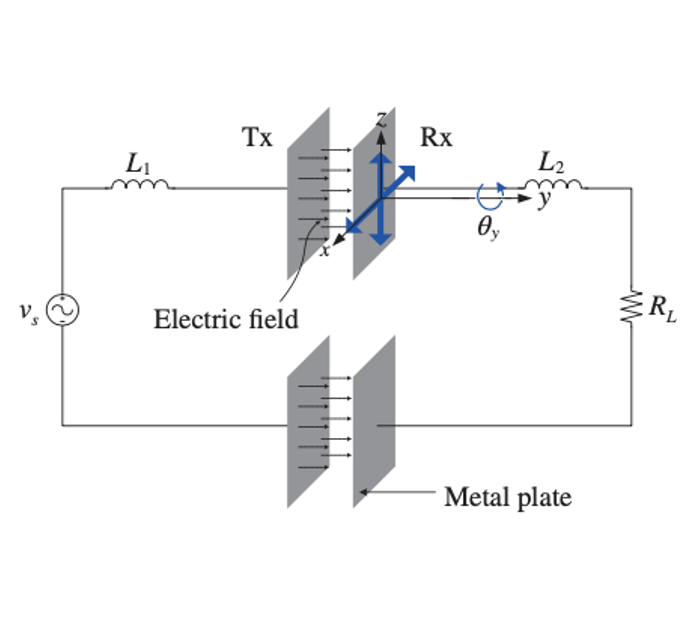
\includegraphics[width=0.9\linewidth]{images/1_capacitive_power_transfer.png}
        \caption{Capacitive power transfer \cite{Chun}.}
        \label{fig:subim1}
    \end{subfigure}
    \begin{subfigure}{0.5\textwidth}
        \centering
        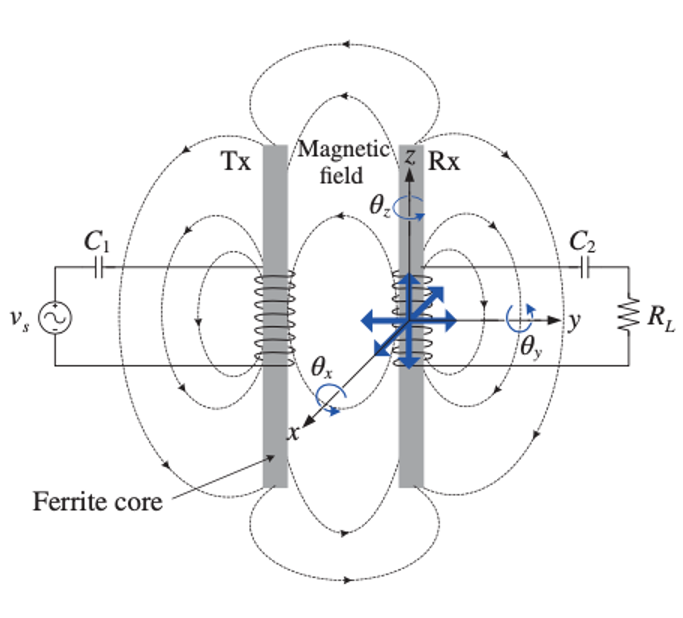
\includegraphics[width=0.9\linewidth]{images/1_inductive_power_transfer.png}
        \caption{Inductive power transfer \cite{Chun}.}
        \label{fig:subim2}
    \end{subfigure}

    \caption{Near-field wireless power transfer.}
    \label{fig:image2}
\end{figure}

\section{Underwater wireless power transfer}



\section{The main research content of this thesis}

\section{Roadmap}